% #######################################
% ########### FILL THESE IN #############
% #######################################
\def\mytitle{LINE ASSIGNMENT}
\def\mykeywords{}
\def\myauthor{SIVA PARVATHI TUNGALA}
\def\contact{tvssn143@gmail.com}
\def\mymodule{ Future Wireless Communication(FWC22089)}
% #######################################
% #### YOU DON'T NEED TO TOUCH BELOW ####
% #######################################
\newcommand{\myvec}[1]{\ensuremath{\begin{pmatrix}#1\end{pmatrix}}}
\let\vec\mathbf
\providecommand{\pr}[1]{\ensuremath{\Pr\left(#1\right)}}
\providecommand{\qfunc}[1]{\ensuremath{Q\left(#1\right)}}
\providecommand{\sbrak}[1]{\ensuremath{{}\left[#1\right]}}
\providecommand{\lsbrak}[1]{\ensuremath{{}\left[#1\right.}}
\providecommand{\rsbrak}[1]{\ensuremath{{}\left.#1\right]}}
\providecommand{\brak}[1]{\ensuremath{\left(#1\right)}}
\providecommand{\lbrak}[1]{\ensuremath{\left(#1\right.}}
\providecommand{\rbrak}[1]{\ensuremath{\left.#1\right)}}
\providecommand{\cbrak}[1]{\ensuremath{\left\{#1\right\}}}
\providecommand{\lcbrak}[1]{\ensuremath{\left\{#1\right.}}
\providecommand{\rcbrak}[1]{\ensuremath{\left.#1\right\}}}
\documentclass[10pt, a4paper]{article}
\usepackage[a4paper,outer=1.5cm,inner=1.5cm,top=1.75cm,bottom=1.5cm]{geometry}
\twocolumn
\usepackage{circuitikz}
\usepackage{amsmath,bm}
\usepackage{amsthm}
\usepackage{mathtools}
\usepackage{amsfonts}
\usepackage{amssymb}
\usepackage{graphicx}
\usepackage{bm}
\newcommand{\bfitDelta}{\bm{\mathit{\Delta}}}

\graphicspath{{./images/}}
%colour our links, remove weird boxes
\usepackage[colorlinks,linkcolor={black},citecolor={blue!80!black},urlcolor={blue!80!black}]{hyperref}
%Stop indentation on new paragraphs
\usepackage[parfill]{parskip}
%% Arial-like font
\usepackage{lmodern}
\renewcommand*\familydefault{\sfdefault}
%Napier logo top right
\usepackage{watermark}
%Lorem Ipusm dolor please don't leave any in you final report ;)
\usepackage{karnaugh-map} 
\usepackage{tabularx}
\usepackage{lipsum}
\usepackage{xcolor}
\usepackage{listings}
%give us the Capital H that we all know and love
\usepackage{float}
%tone down the line spacing after section titles
\usepackage{titlesec}
%Cool maths printing
\usepackage{amsmath}
%PseudoCode
\usepackage{algorithm2e}

\titlespacing{\subsection}{0pt}{\parskip}{-3pt}
\titlespacing{\subsubsection}{0pt}{\parskip}{-\parskip}
\titlespacing{\paragraph}{0pt}{\parskip}{\parskip}
\newcommand{\figuremacro}[5]{
    \begin{figure}[#1]
        \centering
        \includegraphics[width=#5\columnwidth]{#2}
        \caption[#3]{\textbf{#3}#4}
        \label{fig:#2}
    \end{figure}
}


 \lstset{
frame=single, 
breaklines=true,
columns=fullflexible
}
\thiswatermark{\centering \put(1,-110){
\includegraphics[scale=0.05]{iitlogo.jpg}} }
\title{\mytitle}
\author{\myauthor\hspace{1em}\\\contact\\IITH\hspace{0.5em}-\hspace{0.5em}\mymodule}
\date{}
\hypersetup{pdfauthor=\myauthor,pdftitle=\mytitle,pdfkeywords=\mykeywords}
\sloppy
% #######################################
% ########### START FROM HERE ###########
% #######################################
\begin{document}
 \maketitle
 \tableofcontents
 
    
 

 
    
    
    
 
 \Large\section{Problem}
 Q.Straight lines 3x+4y=5 and 4x-3y=15 intersect at point A. Points B and C are choosen on these two lines such that AB=AC. Determine the possible equations of the line BC through the point (1,2).
 
    
   


 \section{Solution}
we know that vector equation of the line is 
\begin{align}
 \textbf{n}^{\top}\textbf{x}=c
\end{align}
The vector equation of the line1 and line2 is
\begin{align}
  \myvec{3 & & 4}\textbf{x}=2
 \\ \myvec{4 & -3}\textbf{x}=3
\end{align}
\centering
\begin{tabular}{|c |c |}
     \hline % <-- Alignments: 1st column left, 2nd middle and 3rd right, with vertical lines in between
	\large\textbf{Symbol} & \large\textbf{Co-ordinates}  \\
       \hline
	\large \textbf{n1} & $\ \begin{pmatrix} 3\\ 4 \end{pmatrix}$  \\
        \hline
	\large \textbf{n2} & $\ \begin{pmatrix} 4\\ -3 \end{pmatrix}$  \\
        \hline
	 \large \textbf{omat} & $\ \begin{pmatrix}0 & 1 \\ -1 & 0 \end{pmatrix}$ \\
       \hline
     \large \textbf{p} & $\ \begin{pmatrix} 1\\ 2 \end{pmatrix}$  \\
        \hline
    \end{tabular}
\\The normal vector for the given vector equations are $ \textbf{n}_{1} \hspace{0.3cm}$and$\hspace{0.3cm}\textbf{n}_{2}. $\\
from (2) and (3) the direction vectors can be written as,
            \\
            \begin{align}
 \textbf{m}_{AB}= \textbf{omat}*\textbf{n}_{1}\\
 \textbf{m}_{AB}=\myvec{4\\ -3} \\
\textbf{m}_{AC}= \textbf{omat}*\textbf{n}_{2}\\
\textbf{m}_{AC}=\myvec{-3\\ -4} \\
\end{align}
from $\bm{\mathit{\Delta}}$ABC,\\
we know that the law of vector addition is given by,\\
\begin{align}
AB+BC=AC\\
\end{align}
By solving (7) we get\\
\begin{align}
\textbf{m}_{BC}=\myvec{-7\\ -1} \\
\end{align}
normal vector for the direction vector BC is,
\begin{align}
\textbf{n}_{3}= \textbf{omat}*\textbf{m}_{BC}\\
\textbf{n}_{3}=\myvec{-1\\ 7} \\
\end{align}
when a line passing through a point the vector equation is,
\begin{align}
\textbf{n}_{3}^{\top}\textbf{(x-p)}=0 \\
\end{align}
By substituting in (16) we get,
\begin{align}
\myvec{-1 & 7}\textbf{x}=13\\
\end{align}
from $\bm{\mathit{\Delta}}$ABC,\\
we know that the law of vector addition is given by,\\
\begin{align}
AB+AC=BC\\
\end{align}
By solving (8) we get\\
\begin{align}
\textbf{m}_{BC}=\myvec{1\\ -7} \\
\end{align}
normal vector for the direction vector BC is,
\begin{align}
\textbf{n}_{4}= \textbf{omat}*\textbf{m}_{BC}\\
\textbf{n}_{4}=\myvec{-7\\ -1} \\
\end{align}
when a line passing through a point the vector equation is,
\begin{align}
\textbf{n}_{4}^{\top}\textbf{(x-p)}=0 \\
\end{align}
By substituting in (25) we get,
\begin{align}
\myvec{7 & 1}\textbf{x}=9\\
\end{align}
  Therefore,the possible equations passing through the point(1,2) are 7y-x=13 and 7x+y=9.

\section{Plot}
\begin{figure}
       \centering
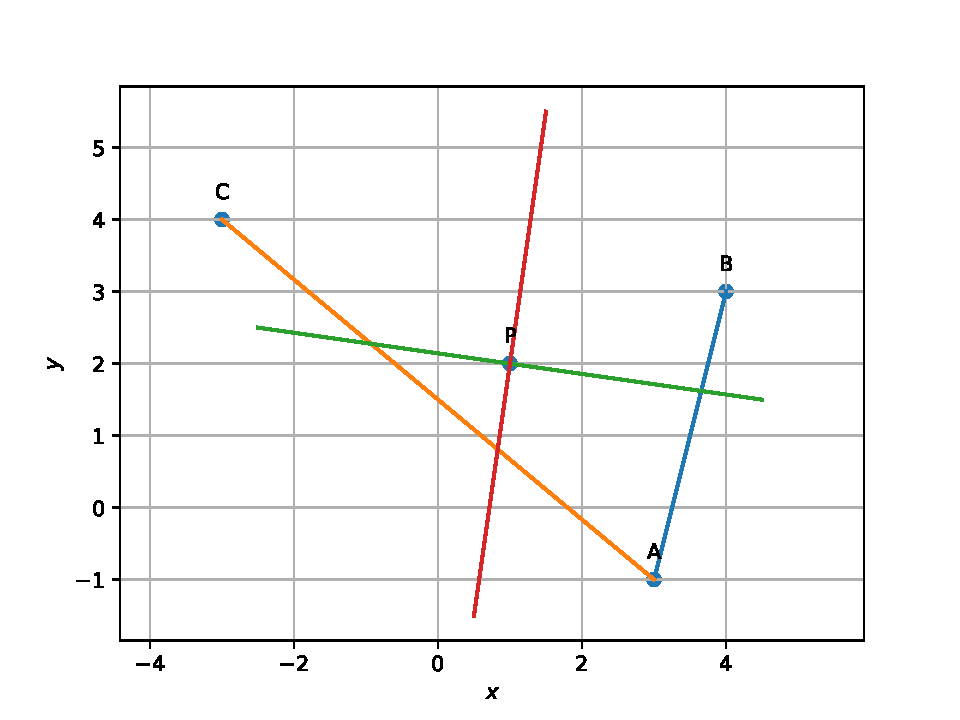
\includegraphics[width=\columnwidth]{fig.pdf}
       \label{fig:my_label}
\end{figure}
        
\section{Software}
  We can get the parallel equation of given equation and the plot of two equtions by executing the following code:
 \vspace{1mm} 
\begin{lstlisting}
https://github.com/sivaparvathi-tungala/fwc_module_1/tree/main/line
\end{lstlisting}
\end{document}
